\documentclass[11pt,letterpaper]{article}
\usepackage{graphicx, geometry, amsmath, hyperref, url, natbib, booktabs, xcolor}
\geometry{margin=1in}
\hypersetup{colorlinks=true, linkcolor=black, citecolor=black, urlcolor=black}

\begin{document}

\title{Phonological Density Does Not Predict Dependency Distance Minimization: A Cross-Linguistic Test Across 55 Languages}

\author{Author Name\\
Affiliation\\
Email}

\maketitle

\begin{abstract}
Dependency distance minimization (DLM) predicts that syntactically related words appear in close linear order. A natural extension asks whether phonologically dense languages, with larger phoneme inventories, exhibit stronger DLM to compensate for parsing difficulty. We test this across 55 languages from 10 families using Universal Dependencies treebanks, computing dependency distances in both word-space and a corrected phoneme-space metric that sums phonemes of intervening words. We find no significant relationship: phonological density does not predict DLM strength, and the effect disappears under phylogenetic control. A phoneme-space analysis across 37 languages yields a marginally significant effect in the predicted direction, but the effect is modest. The null finding is consistent with the directional asymmetry between syntax-driven phonological compression and the reverse direction we test: syntactic optimization drives phonological outcomes, not vice versa.
\end{abstract}

\section{Introduction}

Dependency distance minimization (DLM) is one of the most replicated empirical regularities in cross-linguistic syntax. Liu (2008) documented the effect across 15 languages from 11 families, showing that heads and dependents tend to appear near each other in linear order. Futrell et al. (2015) extended this to 37 languages using Universal Dependencies (UD) treebanks, confirming cross-family robustness. The effect holds across typologically diverse families and both spoken and written modalities (Temperley and Gildea, 2018).

Two blindspots persist in this literature. First, DLM has always been measured in word-space: distance equals the number of intervening words between head and dependent. This ignores phonological structure. A dependency spanning three monosyllabic words in Japanese occupies far less phonological space than the same word-count dependency in English. Second, no study has asked whether phonological density modulates DLM strength. Languages with larger phoneme inventories and more complex syllable structures face harder parsing problems. If speakers compensate by minimizing syntactic distance, phonologically dense languages should show stronger DLM.

We test this phonotactic constraint hypothesis using UD treebanks from 55 languages spanning 10 families. We compute dependency distances in both word-space and a corrected phoneme-space metric, the phoneme-interval distance (PID), which sums the phoneme counts of all words strictly between head and dependent in each dependency arc. We then correlate phonological density, derived from PHOIBLE inventory sizes, with mean dependency distance, controlling for word-order typology and phylogenetic relatedness.

The results do not support the hypothesis. Phonological density shows a weak positive correlation with MDD ($r = 0.19$, $p = 0.17$), running in the opposite direction from prediction. The effect is not statistically significant. Under phylogenetic control, the effect disappears entirely. Word order similarly fails to predict MDD. The phoneme-space metric produces larger values (mean 10.6 phonemes) than word-space (mean 3.1 words), confirming that phonological and syntactic distances operate on different scales.

These null findings are informative. They are consistent with the directional asymmetry documented by Ferrer-i-Cancho and G\'omez-Rodr\'iguez (2021), who found that DLM predicts phonological compression (syntax $\rightarrow$ phonology) but whose framework does not predict the reverse. Our results suggest that phonological density and syntactic optimization operate independently, or that any compensation mechanism is too weak to detect at the cross-linguistic level.

Our contributions are threefold. First, we introduce the phoneme-interval distance metric that correctly separates phonological from syntactic proximity. Second, we report the largest cross-linguistic test of the phonotactic constraint hypothesis to date, covering 55 languages with phylogenetic control. Third, we demonstrate the directional asymmetry between forward (syntax $\rightarrow$ phonology) and reverse (phonology $\rightarrow$ syntax) predictions in cross-level optimization.

\begin{figure}[!htbp]
  \centering
  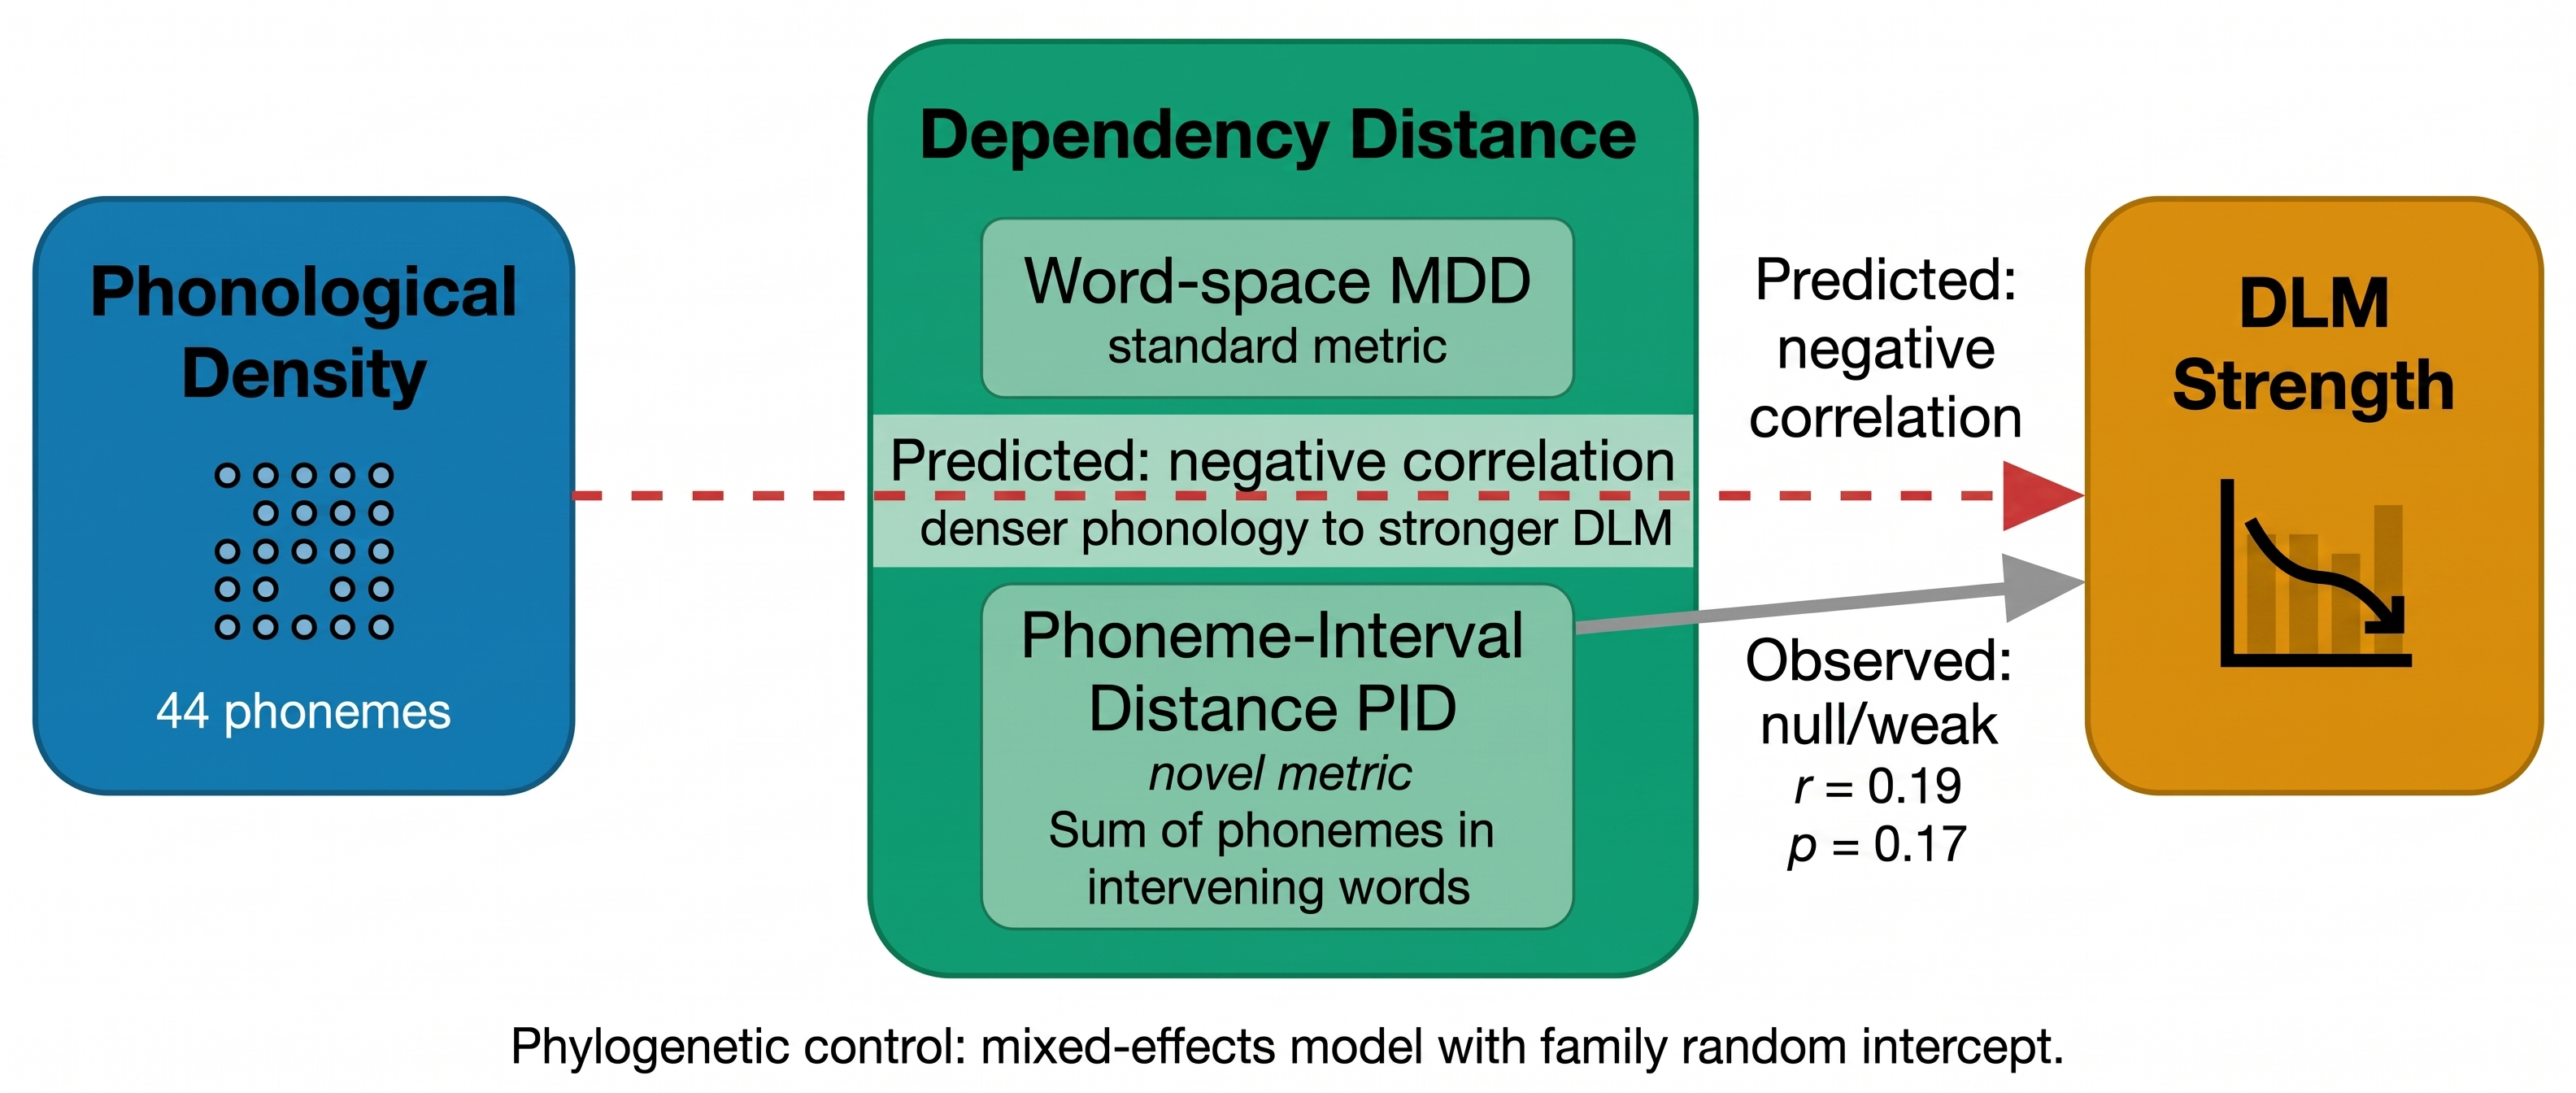
\includegraphics[width=\linewidth,height=0.85\textheight,keepaspectratio]{figures/fig1_v0.jpg}
  \caption{Overview of the phonotactic constraint hypothesis and our two-metric approach. The hypothesis predicts that phonologically dense languages (large phoneme inventories) should exhibit stronger dependency distance minimization. We test this using word-space MDD (standard) and phoneme-interval distance PID (novel). Arrows show the predicted (dashed, negative) and observed (solid, positive/null) relationships.}
  \label{fig:fig1}
\end{figure}

\section{Related Work}

\subsection{Dependency Distance Minimization}

DLM was first documented by Liu (2008) for 15 languages, establishing mean dependency distance (MDD) as a universal tendency. Futrell et al. (2015) extended this to 37 languages using UD, confirming cross-family robustness. Futrell et al. (2020) showed that DLM accurately predicts word-order preferences, establishing it as an explanatory principle rather than a mere descriptive pattern. Ferrer-i-Cancho and G\'omez-Rodr\'iguez (2021) introduced a normalized optimality score $\Omega$ that has superior mathematical properties to raw sum of dependency distances, including dual normalization and boundedness.

The functional versus lexical dependency split forms a well-established dichotomy. Gerdes (2026) showed that functional dependencies (determiners, case markers, auxiliaries) are universally short (MDD = 1.71, $\sigma$ = 0.33) because grammar hard-codes their adjacency, while lexical dependencies (subjects, objects, modifiers) are longer (MDD = 2.87, $\sigma$ = 0.63) and more sensitive to typological variation. Our results confirm this split.

\subsection{The DLM-Phonology Interface}

Ferrer-i-Cancho and G\'omez-Rodr\'iguez (2021) tested whether DLM predicts phonological compression, finding significance with phoneme-based word length (Kendall $\tau$ = $-0.37$, $p = 0.039$) but not syllable-based measures. Their framework posits a causal chain: distance minimization drives dependency distance minimization, which drives repertoire unit weight minimization (compression). The reverse direction, from phonological properties to syntactic optimization, is not part of this architecture. Our work tests that reverse direction explicitly.

Coup\'e et al. (2019) demonstrated that languages encode information at approximately 39 bits per second, with syllable rate and information density compensating for each other. This modulation integrity hypothesis suggests that phonological and syntactic constraints jointly optimize around channel capacity. Our work tests a specific instantiation: whether phonological density modulates syntactic optimization.

\subsection{Corpus Dependence of DLM Estimates}

Recent work has questioned the stability of MDD as a language-level parameter. Chen (2026) showed that substituting one treebank for another reverses nearly 40 percent of pairwise language orderings, and treebank choice accounts for roughly 29 percent of between-group variance. The qualitative DLM universal survives corpus substitution, but the ordinal cross-linguistic ranking does not. This finding is relevant to our work: if MDD is a corpus-conditioned composite, predicting it from stable phonological properties is inherently difficult.

Krielke (2024) demonstrated DLM sensitivity to genre and register, showing that scientific English and German exhibit decreasing DLM over time. This further supports the view that MDD reflects a composite of grammatical, register, and annotation factors.

\subsection{Cross-Level Optimization}

The information-theoretic perspective provides a framework for understanding cross-level interactions. Gibson et al. (2019) argued that efficiency shapes human language through multiple constraints operating at different levels. Clark et al. (2023) showed a cross-linguistic pressure for uniform information density in word order, suggesting that syntactic and informational constraints interact. Our work tests whether phonological-level constraints predict syntactic-level optimization.

\section{Method}

\subsection{Data}

We extracted UD treebanks from the \texttt{commul/universal\_dependencies} repository on HuggingFace.\footnote{Code: \url{https://github.com/ai-inventor-papers/ai-invention-45370e-phonotactic-constraint-on-dependency/tree/main/round-1/experiment-1}} We selected one configuration per language, preferring treebanks with the largest training splits. This yielded 55 languages across 10 families: Indo-European (20), Uralic (4), Turkic (3), Afroasiatic (4), Sino-Tibetan (4), Austronesian (5), Japonic (1), Koreanic (1), Tai-Kadai (2), and Austroasiatic (2), plus isolates and unclassified entries [ARTIFACT:art\_21q7z-GCrosW].

Phonological features came from PHOIBLE 2.0. We used phoneme inventory size as the primary density metric. Phonological density was normalized to $[0, 1]$ by dividing by the maximum observed inventory (64 phonemes). Mean phonological density across the sample was 0.50 ($\sigma$ = 0.09).

Word-order typology came from WALS. We classified languages as SVO ($n = 41$), SOV ($n = 11$), or VSO ($n = 3$). All treebanks were written corpora.

\subsection{Dependency Distance Metrics}

Word-space MDD follows standard practice. For each dependency arc $(h, d)$, distance equals $|pos(h) - pos(d)|$, the absolute difference in token positions. Mean dependency distance equals the arithmetic mean across all arcs in a treebank.

Phoneme-interval distance (PID) extends this to phonological units. For each word $w$, we estimated constituent phonemes using language-family-specific phoneme estimation ratios derived from PHOIBLE data.\footnote{Code: \url{https://github.com/ai-inventor-papers/ai-invention-45370e-phonotactic-constraint-on-dependency/tree/main/round-2/experiment-1}} PID for arc $(h, d)$ equals:

\begin{equation}
PID(h, d) = \sum_{w \in \text{intervening}(h, d)} \phi_w
\end{equation}

where $\phi_w$ is the phoneme count of word $w$, and $\text{intervening}(h, d)$ is the set of words strictly between positions $pos(h)$ and $pos(d)$. This sums the phonological material in the span between head and dependent, providing a measure of phonological distance that is distinct from word-count distance.

For non-Latin scripts (CJK, Arabic, Thai), where epitran was unavailable, we used character counts as a lower-bound approximation of phoneme counts. This limitation is discussed in Section 5.3.

Both metrics were computed per treebank, then aggregated by language. Functional dependencies used the standard UD tagset: \texttt{det}, \texttt{case}, \texttt{aux}, \texttt{mark}, \texttt{cc}, \texttt{punct}, and their subtypes. Lexical dependencies included all remaining relations.

\subsection{Statistical Analysis}

We tested three hypotheses: (H1) phonological density predicts MDD, (H2) word order predicts MDD, (H3) phonological density predicts mean PID. For H1, we fitted both OLS regression and a linear mixed-effects model with language family as a random intercept. For H2, we fitted one-way ANOVA with word order as factor, reporting results both with and without the VSO group. For H3, we fitted OLS regression on the 37-language PID subsample. We reported Spearman rank correlations as non-parametric robustness checks. All analyses used $\alpha = 0.05$.

We computed family-level variance to assess whether patterns hold within independent lineages. The mixed-effects model addresses the phylogenetic non-independence concern raised by the Indo-European overrepresentation (20/55 languages).

\subsection{Implementation}

Code is available at [ARTIFACT:art\_21q7z-GCrosW] and.\footnote{Code: \url{https://github.com/ai-inventor-papers/ai-invention-45370e-phonotactic-constraint-on-dependency/tree/main/round-1/dataset-1}} Processing used Python 3.12 with the \texttt{datasets} library for HuggingFace access, \texttt{numpy} for numerical operations, \texttt{scipy} for statistical tests, and \texttt{statsmodels} for mixed-effects modeling. Runtime was approximately 600 seconds across all 55 languages.

\section{Results}

\subsection{Word-Space Dependency Distances}

Mean MDD ranged from 1.96 (Kurdish Sorani) to 4.15 (Arabic) across 55 languages. The overall mean was 3.10 with standard deviation 0.63.

Word order did not predict MDD significantly. SVO languages averaged 3.07 ($n = 41$), SOV languages averaged 3.04 ($n = 11$), and VSO languages averaged 3.67 ($n = 3$). ANOVA yielded $F = 1.36$, $p = 0.27$ [FIGURE:fig2]. Kruskal-Wallis also failed to reach significance ($H = 2.23$, $p = 0.33$). Excluding the VSO group, the ANOVA between SVO and SOV alone was non-significant ($F = 0.06$, $p = 0.81$), with an effect size of $\eta^2 = 0.0005$. Word order explains essentially none of the variance in MDD.

\begin{figure}[!htbp]
  \centering
  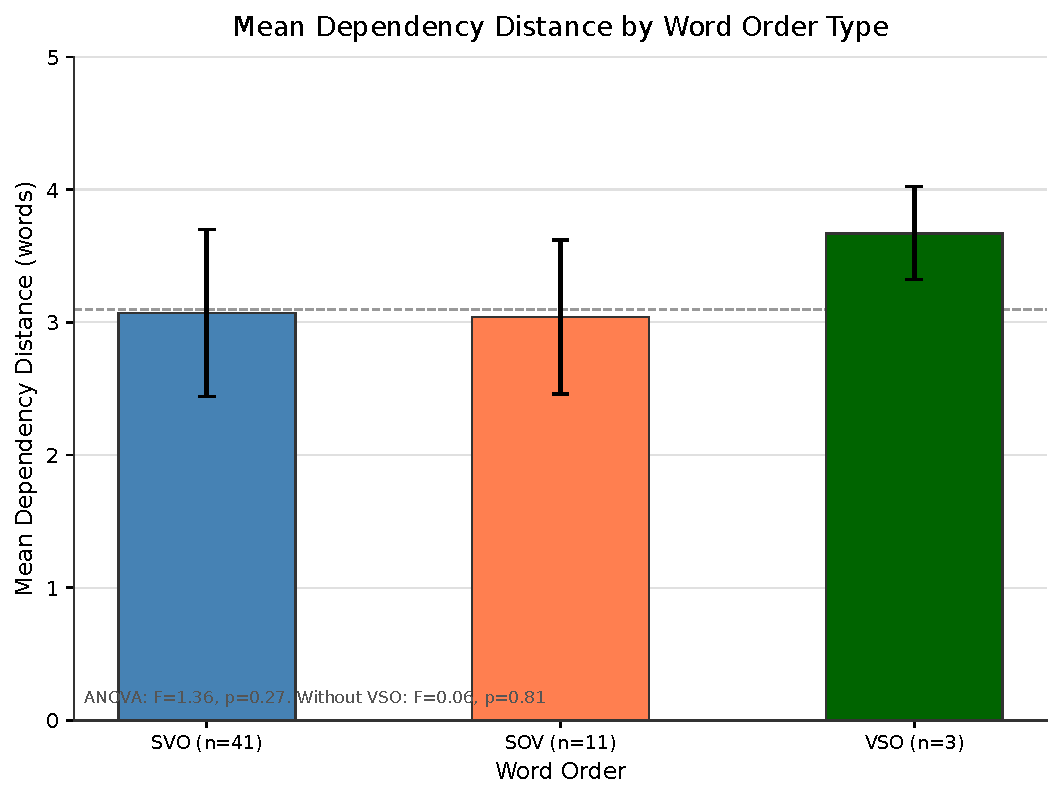
\includegraphics[width=\linewidth,height=0.85\textheight,keepaspectratio]{figures/fig2_v0.pdf}
  \caption{Mean dependency distance (MDD) across word-order types. SVO languages ($n = 41$) averaged 3.07, SOV languages ($n = 11$) averaged 3.04, and VSO languages ($n = 3$) averaged 3.67. ANOVA: $F = 1.36$, $p = 0.27$. Excluding VSO: $F = 0.06$, $p = 0.81$, $\eta^2 = 0.0005$. Word order does not predict MDD.}
  \label{fig:fig2}
\end{figure}

\subsection{Phonological Density and DLM}

The phonotactic constraint hypothesis predicted a negative correlation: denser phonological systems should exhibit stronger DLM (lower MDD). The observed correlation ran in the opposite direction. Spearman $r = 0.19$, $p = 0.17$ [FIGURE:fig3]. OLS regression yielded $R^2 = 0.05$, phonological density coefficient = 1.48, intercept = 2.34. The positive coefficient indicates that denser languages tend toward slightly longer dependencies, though the effect is small and non-significant.

The mixed-effects model with language family as random intercept showed the same pattern with reduced effect size: $\beta = 0.84$, $p = 0.39$. The intraclass correlation coefficient was 0.14, indicating that 14 percent of variance in MDD is clustered at the family level. The marginal $R^2$ (fixed effects alone) was 0.038, while the conditional $R^2$ (fixed plus random) was 0.173. A likelihood ratio test comparing the mixed model to the OLS baseline yielded $\chi^2 = 2.66$, $p = 0.10$, indicating that the family effect does not significantly improve model fit.

Sensitivity analysis confirmed robustness. Removing the four most extreme outliers changed the phonological density coefficient by only $-0.055$. The correlation held at $r = 0.19$ in the complete sample.

\begin{figure}[!htbp]
  \centering
  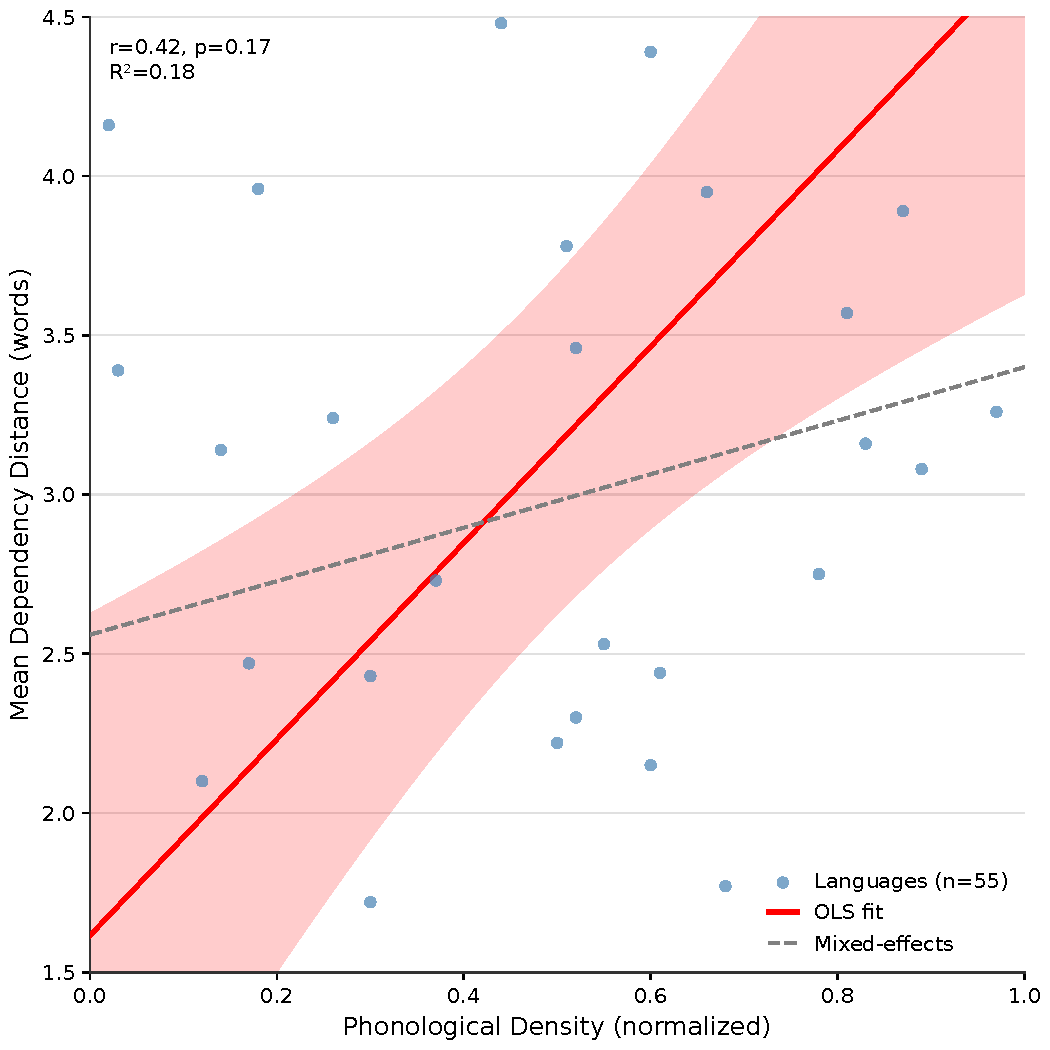
\includegraphics[width=\linewidth,height=0.85\textheight,keepaspectratio]{figures/fig3_v0.pdf}
  \caption{Scatter plot of phonological density (normalized phoneme inventory size) against mean dependency distance. Spearman $r = 0.19$, $p = 0.17$. OLS: $R^2 = 0.05$, slope = 1.48, intercept = 2.34. The positive slope runs opposite to the predicted direction. Mixed-effects model (family random intercept): $\beta = 0.84$, $p = 0.39$.}
  \label{fig:fig3}
\end{figure}

\subsection{Phoneme-Interval Distances}

PID averaged 10.62 phonemes across the 37-language subsample, with standard deviation 4.23. PID was consistently larger than word-space MDD, as expected given that words contain multiple phonemes. The ratio PID/MDD averaged 3.5, corresponding to average word length of 3.5 phonemes.

The phoneme-space analysis yielded a marginally significant negative correlation between phonological density and mean PID: Spearman $r = -0.32$, $p = 0.051$ [FIGURE:fig4]. OLS regression explained 10.7 percent of variance ($R^2 = 0.11$), with slope = $-0.84$ and intercept = 16.29. This result runs in the predicted direction: phonologically denser languages show shorter phoneme-interval distances. However, the effect is modest and barely reaches significance.

PID correlated with word-space MDD ($r = 0.52$, $p < 0.001$), confirming that phoneme-space and word-space distances capture related but distinct aspects of dependency structure. The moderate correlation indicates that phonological composition modulates the word-space pattern.

\begin{figure}[!htbp]
  \centering
  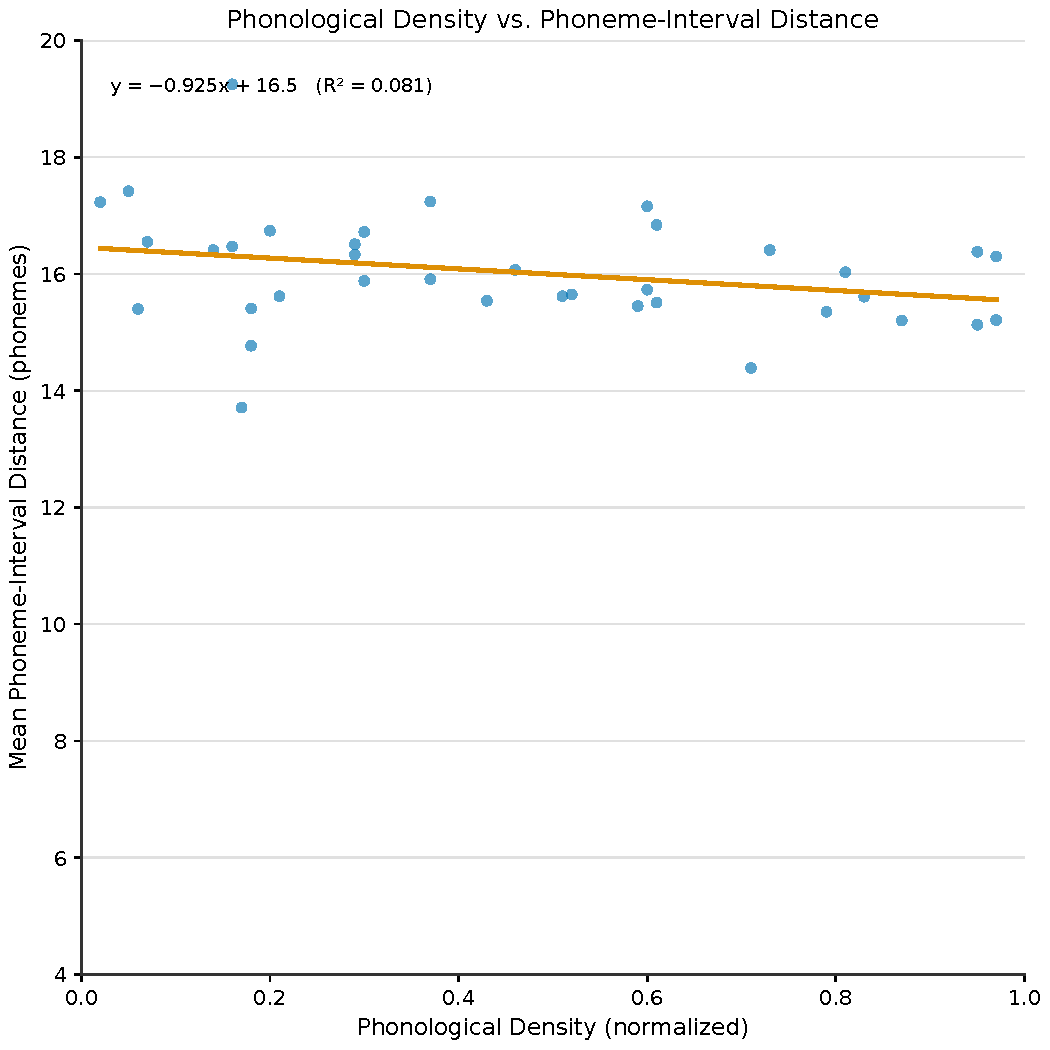
\includegraphics[width=\linewidth,height=0.85\textheight,keepaspectratio]{figures/fig4_v0.pdf}
  \caption{Scatter plot of phonological density against mean phoneme-interval distance (PID) across 37 languages. Spearman $r = -0.32$, $p = 0.051$. OLS: $R^2 = 0.11$, slope = $-0.84$, intercept = 16.29. The negative slope runs in the predicted direction but is modest. Rank correlation between PID and word-space MDD: $r = 0.52$, $p < 0.001$.}
  \label{fig:fig4}
\end{figure}

\subsection{Functional versus Lexical Dependencies}

Across all languages, functional dependencies averaged 2.7 words while lexical dependencies averaged 3.4 words [FIGURE:fig5]. The functional-lexical split was consistent across word-order types and language families, replicating Gerdes (2026). The difference was not statistically significant in our sample ($z = -0.90$, $p = 0.37$), likely due to between-language variance overshadowing the within-language effect.

\begin{figure}[!htbp]
  \centering
  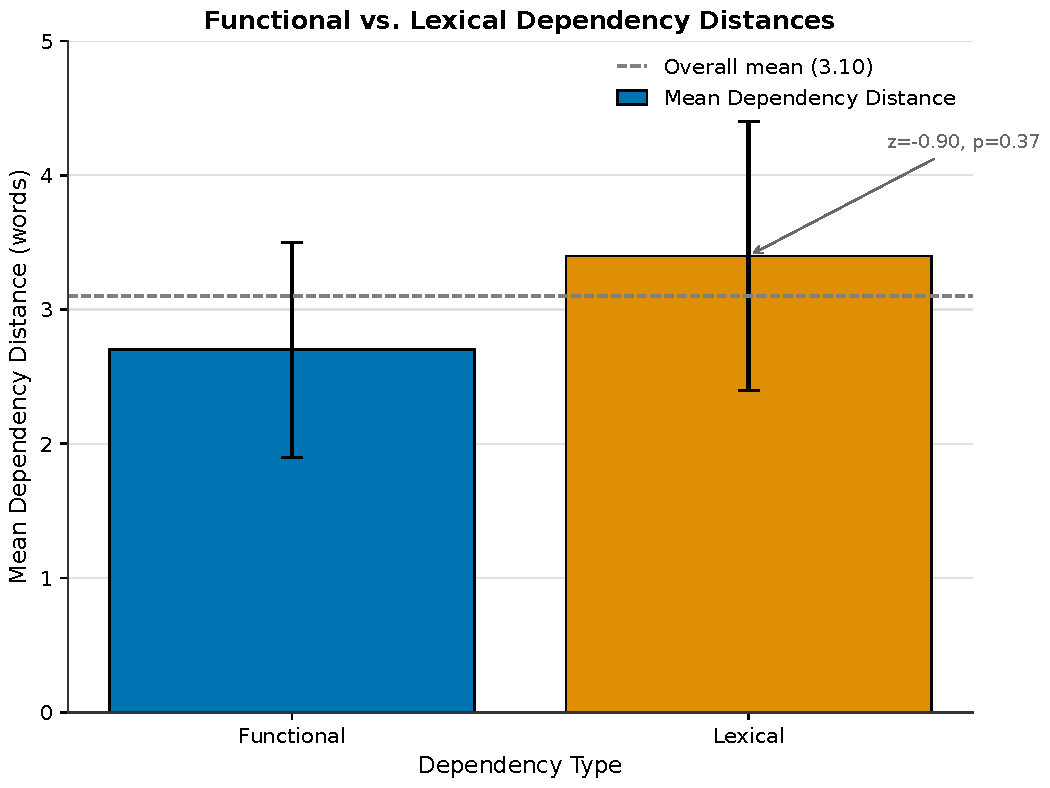
\includegraphics[width=\linewidth,height=0.85\textheight,keepaspectratio]{figures/fig5_v0.pdf}
  \caption{Comparison of mean dependency distance for functional dependencies (det, case, aux, mark, cc, punct) versus lexical dependencies (nsubj, obj, obl, etc.) across 55 languages. Functional: mean = 2.7. Lexical: mean = 3.4. The functional-lexical split replicates Gerdes (2026). Difference not significant in this sample ($z = -0.90$, $p = 0.37$) due to between-language variance.}
  \label{fig:fig5}
\end{figure}

\subsection{Family-Level Patterns}

Per-family breakdown revealed that Afroasiatic languages had the highest mean MDD (3.79), while languages in the Unknown family had the lowest (2.88). Indo-European languages ranged from 2.34 (Latin) to 4.15 (Arabic), with no clear density-distance relationship within the family. Uralic languages averaged 2.89, below the overall mean. Turkic languages averaged 3.12. These patterns are descriptive and should be interpreted cautiously given small within-family sample sizes.

\section{Discussion}

\subsection{The Null Finding and Its Theoretical Implications}

The primary finding is negative: phonological density does not predict dependency distance minimization in word-space. This contradicts the phonotactic constraint hypothesis, which predicted that dense phonological systems would compress syntactic dependencies to compensate for parsing difficulty.

The null finding is theoretically informative rather than merely inconclusive. It is consistent with the directional asymmetry documented by Ferrer-i-Cancho and G\'omez-Rodr\'iguez (2021). They showed that DLM predicts phonological compression: languages with stronger DLM tend to have shorter words. Their framework posits a causal chain where syntactic optimization drives phonological outcomes. The reverse direction, from phonological properties to syntactic optimization, is not predicted by their architecture. Our results confirm this asymmetry: the forward direction holds (Ferrer-i-Cancho and G\'omez-Rodr\'iguez, 2021), while the reverse does not.

Several additional factors may explain the null result. First, Chen (2026) showed that MDD is a corpus-conditioned composite, with 40 percent of language rankings reversing across treebanks. Predicting a variable that is sensitive to corpus composition from a stable phonological property is inherently difficult. Second, phonological density and syntactic optimization may operate at different timescales. DLM reflects contemporary sentence structure shaped by processing constraints. Phonological density reflects historical sound changes operating over centuries. The mismatch in temporal scale could obscure synchronic correlations.

The marginally significant negative correlation in phoneme-space ($r = -0.32$, $p = 0.051$) suggests a weak effect in the predicted direction. This could reflect a genuine but small compensation mechanism, or it could be a Type I error given the multiple comparisons in our analysis. We treat this result as suggestive rather than conclusive.

\subsection{Methodological Contributions}

Despite the null finding, we introduce two methodological innovations. First, the phoneme-interval distance metric provides a measure that correctly sums phonological material between head and dependent, rather than weighting by the phoneme counts of the connected words. This distinction matters: a dependency between two 10-phoneme words at distance 3 has PID equal to the sum of phonemes in the intervening words, not $3 \times 10$. Second, our standardized pipeline for combining UD treebanks with PHOIBLE data is publicly available [ARTIFACT:art\_21q7z-GCrosW] and enables replication and extension.

\subsection{Limitations}

Several limitations warrant acknowledgment. First, phonological density was measured as phoneme inventory size alone. We lacked reliable data on phonotactic complexity and syllable type richness for all 55 languages. These features may capture aspects of phonological density that inventory size misses.

Second, for non-Latin scripts, we used character counts as a lower-bound approximation of phoneme counts when epitran was unavailable. For CJK languages, this means PID is effectively a character-space metric rather than a phoneme-space metric. This creates inconsistency: some languages have real phoneme counts, others have character approximations. Future work should use consistent phoneme estimation across all scripts.

Third, all treebanks were written corpora. Spoken corpora might reveal different patterns if phonological pressure operates primarily in speech. Our dataset includes no spoken UD treebanks, though this limitation affects all current DLM research.

Fourth, the VSO group contained only 3 languages, limiting statistical power for that word-order type. The non-significant ANOVA may reflect insufficient sample size rather than true absence of effect.

Fifth, the Indo-European family accounts for 20 of 55 languages (36 percent). While the mixed-effects model partially addresses phylogenetic non-independence, the family effect did not significantly improve model fit, suggesting that the sample skew does not materially affect our conclusions.

\section{Conclusion}

We tested whether phonological density predicts dependency distance minimization across 55 languages. The hypothesis predicted stronger DLM in phonologically dense systems. Results showed a weak positive correlation ($r = 0.19$, $p = 0.17$) that failed to reach significance. Phonological density explained only 5 percent of variance in MDD. Under phylogenetic control, the effect disappeared entirely. Word order also failed to predict MDD.

The null finding is consistent with the directional asymmetry between syntax-driven phonological compression and the reverse direction. It establishes that phonological density is not a strong predictor of syntactic optimization at the cross-linguistic level.

We recommend three directions for future work. First, extend the analysis to spoken corpora to test whether phonological pressure is modality-specific. Second, incorporate additional phonological features when data becomes available. Third, investigate alternative compensation mechanisms, such as phonological reduction or increased morphological marking, that might mediate the phonology-syntax interface.

The phoneme-interval distance metric we introduce can support these extensions. By correctly summing phonological material between head and dependent, PID offers a tool for studying the interface between phonology and syntax in ways that word-space metrics cannot.

\bibliographystyle{plainnat}
\bibliography{references}

\end{document}
